\input{preamble.tex}
\title{Отчет по лабораторной работе № 6. \\ Адресация IPv4 и IPv6. Двойной стек }
\author{Данила Стариков \\ НПИбд-02-22}
\date{2024}

\begin{document}

\maketitle
\newpage

\tableofcontents

\newpage
\section{Цель работы}
Изучение принципов распределения и настройки адресного пространства на устройствах сети.
\newpage
\section{Выполнение работы}
\subsection{Настройка двойного стека адресации IPv4 и IPv6 в локальной сети}
\subsubsection{Постановка задачи}
Задана топология сети с двумя локальными подсетями (рис. \ref{28}). Для первой подсети выделено адресное пространство с адресами IPv4, для второй — адресное пространство с адресами IPv6 (табл. \ref{tab1}).

\begin{center}
    \centering
    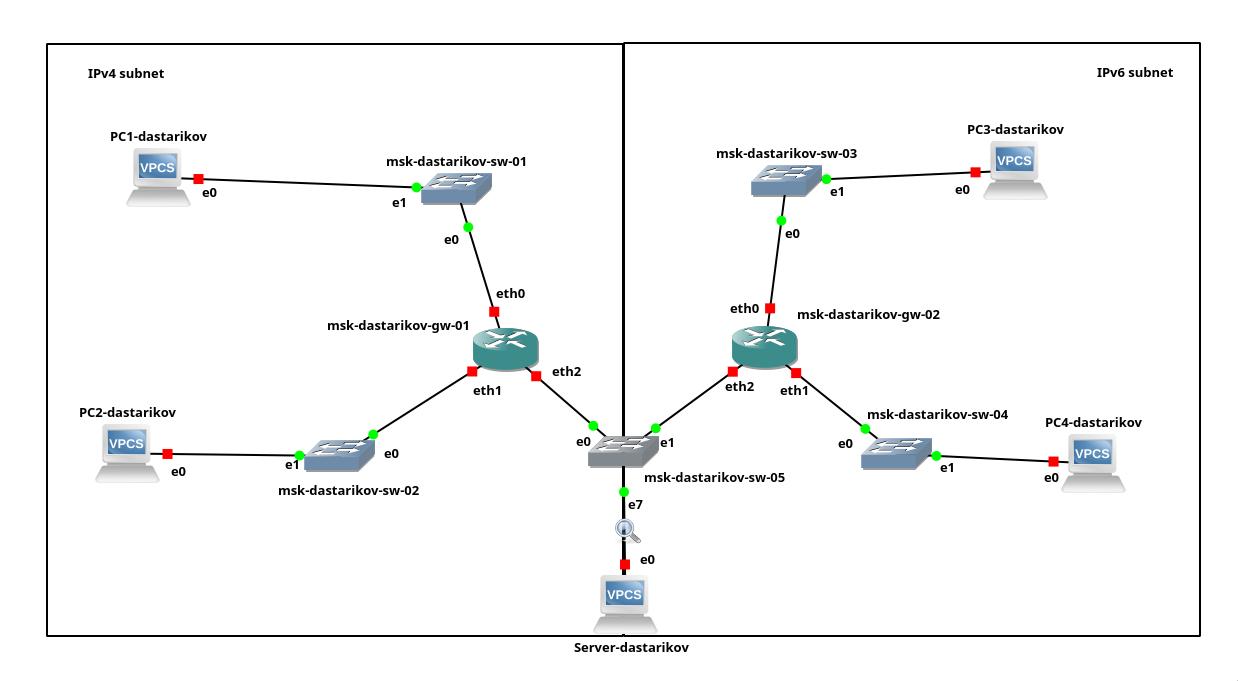
\includegraphics[width=\textwidth]{../images/image28.png}
    \captionof{figure}{Топология сети.}
    \label{28}
\end{center}


Требуется:
\begin{itemize}
\item реализовать топологию сети в GNS3;
\item настроить IPv4-адресацию на устройствах первой подсети и проверить подключение между устройствами этой подсети;
\item настроить IPv6-адресацию на устройствах второй подсети и проверить подключение между устройствами этой подсети;
\item проанализировать захваченный на соединении сервера двойного стека адресации с коммутатором трафик ARP, ICMP, ICMPv6.
\end{itemize}

\begin{table}[]
  \centering
  \caption{Таблица адресации}
  \label{tab1}
\begin{tabular}{|llll|}
\hline
\multicolumn{1}{|l|}{Устройство} & \multicolumn{1}{l|}{Интерфейс} & \multicolumn{1}{l|}{IPv4-адрес} & Шлюз по умолчанию \\ \hline
gw-01                            & eth0                           & 172.16.20.1/25                  &                   \\
gw-01                            & eth1                           & 172.16.20.129/25                &                   \\
gw-01                            & eth2                           & 64.100.1.1/24                   &                   \\ \hline
PC1                              & NIC                            & 172.16.20.10/25                 & 172.16.20.1       \\
PC2                              & NIC                            & 172.16.20.138/25                & 172.16.20.129     \\ \hline
gw-02                            & eth0                           & 2001:db8:c0de:12::1/64          &                   \\
gw-02                            & eth1                           & 2001:db8:c0de:13::1/64          &                   \\
gw-02                            & eth2                           & 2001:db8:c0de:11::1/64          &                   \\ \hline
PC3                              & NIC                            & 2001:db8:c0de:12::a/64          & gw-02             \\
PC4                              & NIC                            & 2001:db8:c0de:13::a/64          & gw-02             \\ \hline
Server                           & NIC                            & 64.100.1.10/24                  & 64.100.1.1        \\
Server                           & NIC                            & 2001:db8:c0de:11::a/64          & gw-02             \\ \hline
\end{tabular}
\end{table}
\subsubsection{Порядок выполнения работы}
\begin{enumerate}
\item Запустили GNS3 VM и GNS3. Создали новый проект.
\item В рабочем пространстве разместили и соединили устройства в соответствии с топологией, приведённой на рис. \ref{28}. Для обеих подсетей IPv4 использовали маршрутизаторы Vyos.

\item Изменили отображаемые названия устройств. Коммутаторам присвоили названия по принципу \texttt{msk-dastarikov-sw-0x}, маршрутизаторам — по принципу \texttt{msk-dastarikov-gw-0x}, VPCS — по принципу \texttt{PCx-dastarikov}, вместо \texttt{x} — порядковый номер устройства.
\item Включили захват трафика на соединении между сервером двойного стека адресации и ближайшим к нему коммутатором.
\item Руководствуясь табл. \ref{tab1}, настроили IPv4-адресацию для интерфейсов узлов PC1, PC2, Server:
  – PC1 (рис. \ref{01}):
  \begin{minted}{bash}
    ip 172.16.20.10/25 172.16.20.1
    save
  \end{minted}

\begin{center}
    \centering
    
\includegraphics[width=\textwidth]{../images/image01.png}
    \captionof{figure}{Настройка IP-адреса на PC1.}
    \label{01}
\end{center}

  – PC2 (рис. \ref{02}):
  \begin{minted}{bash}
    ip 172.16.20.138/25 172.16.20.129
    save
  \end{minted}

\begin{center}
    \centering
    
\includegraphics[width=\textwidth]{../images/image02.png}
    \captionof{figure}{Настройка IP-адреса на PC2.}
    \label{02}
\end{center}

  – Server (рис. \ref{03}):
  \begin{minted}{bash}
    ip 64.100.1.10/24 64.100.1.1
    save
  \end{minted}

\begin{center}
    \centering
    
\includegraphics[width=\textwidth]{../images/image03.png}
    \captionof{figure}{Настройка IP-адреса на Server.}
    \label{03}
\end{center}

  – Посмотрели на PC1 и PC2 конфигурацию IPv4 и IPv6 (рис. \ref{04} и \ref{05}):
  \begin{minted}{bash}
    show ip
    show ipv6
  \end{minted}

\begin{center}
    \centering
    
\includegraphics[width=\textwidth]{../images/image04.png}
    \captionof{figure}{Просмотр конфигурации IPv4 и IPv6 на PC1.}
    \label{04}
\end{center}

\begin{center}
    \centering
    
\includegraphics[width=\textwidth]{../images/image05.png}
    \captionof{figure}{Просмотр конфигурации IPv4 и IPv6 на PC2.}
    \label{05}
\end{center}

\item Руководствуясь табл. \ref{tab1} настроили IPv4-адресацию для интерфейсов локальной сети маршрутизатора VyOS \texttt{msk-dastarikov-gw-01} (рис. \ref{07}):

\begin{center}
    \centering
    
\includegraphics[width=\textwidth]{../images/image07.png}
    \captionof{figure}{Настройка IP-адреса на маршрутизаторе \texttt{gw-01}.}
    \label{07}
\end{center}

\item Проверили конфигурацию маршрутизатора и настройки IPv4-адресации (рис. \ref{09}):
  
\begin{center}
    \centering
    
\includegraphics[width=\textwidth]{../images/image09.png}
    \captionof{figure}{Просмотр конфигурации на маршрутизаторе \texttt{gw-01}.}
    \label{09}
\end{center}

\item Проверили подключение с помощью команд \texttt{ping} и \texttt{trace}. Узлы PC1 и PC2 должны успешно отправлять эхо-запросы друг другу и на сервер с двойным стеком (Dual Stack Server) (рис. \ref{11}).

\begin{center}
    \centering
    
\includegraphics[width=\textwidth]{../images/image11.png}
    \captionof{figure}{Проверка подключения между узлами PC1, PC2 и сервером сети.} 
    \label{11}
\end{center}

\item Руководствуясь табл. \ref{tab1}, настроили IPv6-адресацию для интерфейсов узлов PC3, PC4, Server:
  – PC3 (рис. \ref{12}):
  \begin{minted}{bash}
    ip 2001:db8:c0de:12::a/64
    save
  \end{minted}

\begin{center}
    \centering
    
\includegraphics[width=\textwidth]{../images/image12.png}
    \captionof{figure}{Настройка IP-адреса на PC3.}
    \label{12}
\end{center}

  – PC4 (рис. \ref{13}):
  \begin{minted}{bash}
    ip 2001:db8:c0de:13::a/64
    save
  \end{minted}

\begin{center}
    \centering
    
\includegraphics[width=\textwidth]{../images/image13.png}
    \captionof{figure}{Настройка IP-адреса на PC4.}
    \label{13}
\end{center}

  – Server (рис. \ref{14}):
  \begin{minted}{bash}
    ip 2001:db8:c0de:11::a/64
    save
  \end{minted}

\begin{center}
    \centering
    
\includegraphics[width=\textwidth]{../images/image14.png}
    \captionof{figure}{Настройка IPv6-адреса на Server.}
    \label{14}
\end{center}

\item Посмотрели на PC3 и PC4 конфигурацию IPv4 и IPv6 (рис. \ref{15} и \ref{16}):
  \begin{minted}{bash}
    show ip
    show ipv6
  \end{minted}

\begin{center}
    \centering
    
\includegraphics[width=\textwidth]{../images/image15.png}
    \captionof{figure}{Просмотр конфигурации Server.}
    \label{15}
\end{center}

\begin{center}
    \centering
    
\includegraphics[width=\textwidth]{../images/image16.png}
    \captionof{figure}{Просмотр конфигурации PC3.}
    \label{16}
\end{center}

\item Руководствуясь табл. \ref{tab1}, настроили IPv6-адресацию для интерфейсов локальной сети маршрутизатора VyOS \texttt{msk-dastarikov-gw-02}:

  \begin{itemize}
  \item Перешли в режим конфигурирования, изменили имя устройства (рис. \ref{17}):
    \begin{minted}{bash}
      vyos@vyos$ configure
      vyos@vyos# set system host-name msk-dastarikov-gw-02
      vyos@vyos# compare
      vyos@vyos# commit
      vyos@vyos# save
      vyos@vyos# exit
      vyos@vyos$ reboot
    \end{minted}

\begin{center}
    \centering
    
\includegraphics[width=\textwidth]{../images/image17.png}
    \captionof{figure}{Настройка имени устройства.}
    \label{17}
\end{center}

  \item Назначили IPv6-адреса маршрутизатору \texttt{msk-dastarikov-gw-02} (рис. \ref{18}):
    \begin{minted}{bash}
      vyos@msk-dastarikov-gw-02:~$ configure
      vyos@msk-dastarikov-gw-02# set interfaces ethernet eth0 address 2001:db8:c0de:12::1/64
      vyos@msk-dastarikov-gw-02# set service router-advert interface eth0 prefix 2001:db8:c0de:12::/64
      vyos@msk-dastarikov-gw-02# set interfaces ethernet eth1 address 2001:db8:c0de:13::1/64
      vyos@msk-dastarikov-gw-02# set service router-advert interface eth1 prefix 2001:db8:c0de:13::/64
      vyos@msk-dastarikov-gw-02# set interfaces ethernet eth2 address 2001:db8:c0de:11::1/64
      vyos@msk-dastarikov-gw-02# set service router-advert interface eth2 prefix 2001:db8:c0de:11::/64
      vyos@msk-dastarikov-gw-02# compare
      vyos@msk-dastarikov-gw-02# commit
      vyos@msk-dastarikov-gw-02# save
      vyos@msk-dastarikov-gw-02# show interfaces
    \end{minted}

\begin{center}
    \centering
    
\includegraphics[width=\textwidth]{../images/image18.png}
    \captionof{figure}{Конфигурация машрутизатора \texttt{gw-02}.}
    \label{18}
  \end{center}
\end{itemize}

\item Проверили подключение с помощью команд \texttt{ping} и \texttt{trace}. Узлы PC3 и PC4 должны успешно отправлять эхо-запросы друг другу и на сервер с двойным стеком (Dual Stack Server) (рис. \ref{19} и \ref{20}).

\begin{center}
    \centering
    
\includegraphics[width=\textwidth]{../images/image19.png}
    \captionof{figure}{Проверка подключения узла PC3 к узлам PC4 и серверу.}
    \label{19}
\end{center}

\begin{center}
    \centering
    
\includegraphics[width=\textwidth]{../images/image20.png}
    \captionof{figure}{Проверка подключения узла PC4 к узлам PC3 и серверу.}
    \label{20}
\end{center}

\item Убедились, что устройства из подсети IPv4 не доступны для устройств из подсети IPv6 и наоборот. Только сервер двойного стека может обращаться к устройствам обеих подсетей (рис. \ref{21}-\ref{24}).

\begin{center}
    \centering
    
\includegraphics[width=\textwidth]{../images/image21.png}
    \captionof{figure}{Попытка подключения к узлам PC3 и PC4 с PC1.}
    \label{21}
\end{center}

\begin{center}
    \centering
    
\includegraphics[width=\textwidth]{../images/image22.png}
    \captionof{figure}{Попытка подключения к узлам PC3 и PC4 с PC2.}
    \label{22}
\end{center}

\begin{center}
    \centering
    
\includegraphics[width=\textwidth]{../images/image23.png}
    \captionof{figure}{Попытка подключения к узлам PC1 и PC1 с PC3.}
    \label{23}
\end{center}

\begin{center}
    \centering
    
\includegraphics[width=\textwidth]{../images/image24.png}
    \captionof{figure}{Попытка подключения к узлам PC1 и PC2 с PC4.}
    \label{24}
\end{center}

\item Посмотрели захваченный на соединении сервера двойного стека адресации с коммутатором трафик ARP, ICMP, ICMPv6 (рис. \ref{26} и \ref{27}).

\begin{center}
    \centering
    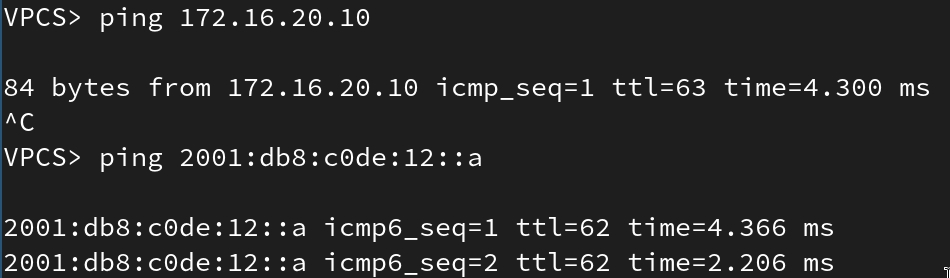
\includegraphics[width=\textwidth]{../images/image26.png}
    \captionof{figure}{Отправка эхо-запроса с сервера к PC1.}
    \label{26}
\end{center}

\begin{center}
    \centering
    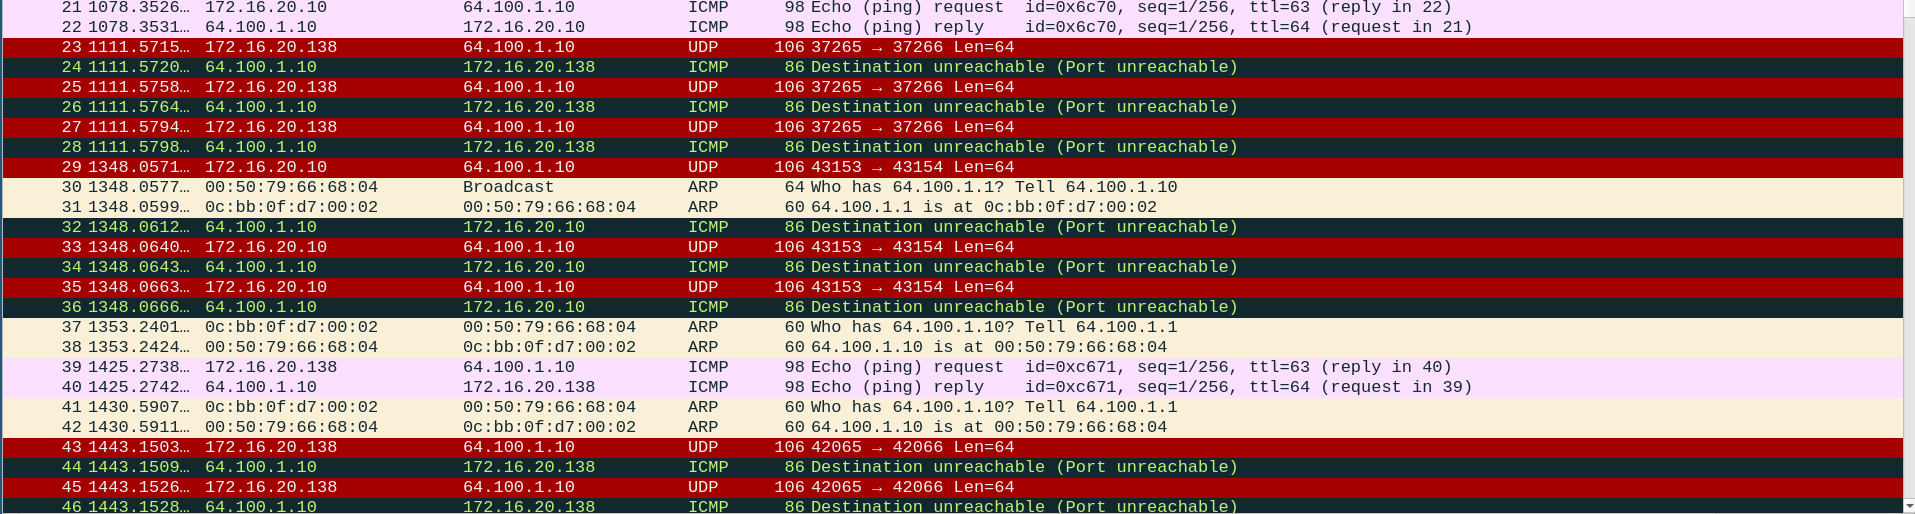
\includegraphics[width=\textwidth]{../images/image27.png}
    \captionof{figure}{Просмотр перехваченных пакетов.}
    \label{27}
\end{center}
\end{enumerate}

\subsection{Задание для самостоятельного выполнения}

\subsubsection{Постановка задачи}

Задана топология сети (рис. \ref{37}).

\begin{center}
    \centering
    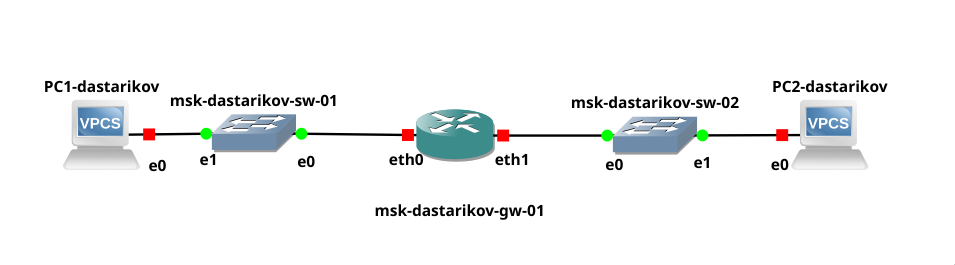
\includegraphics[width=\textwidth]{../images/image37.png}
    \captionof{figure}{Топология сети.}
    \label{37}
\end{center}

Предполагается, что маршрутизатор разбивает сеть на две подсети с адресами IPv4 и IPv6:
\begin{itemize}
\item подсеть 1: 10.10.1.96/27; 2001:DB8:1:1::/64;
\item подсеть 2: 10.10.1.16/28; 2001:DB8:1:4::/64.
\end{itemize}
Требуется:
\begin{enumerate}
\item Охарактеризовать подсети, указать, какие адреса в них входят.
\item Предложить вариант таблицы адресации для заданной топологии и адресного пространства, причём для интерфейсов маршрутизатора выбрать наименьший адрес в подсети.
\item Настроить IP-адресацию на маршрутизаторе VyOS и оконечных устройствах, причём на интерфейсах маршрутизатора установить наименьший адрес в подсети.
\item Проверить подключение между устройствами подсети с помощью команд \texttt{ping} и \texttt{trace}.
\end{enumerate}

\subsubsection{Выполнение}

\begin{enumerate}

\item Составили таблицу адресации для моделируемой сети (табл. \ref{tab2}):

\begin{table}[]
\centering
\caption{Таблица адресации}
\label{tab2}
\begin{tabular}{|l|l|l|l|l|}
\hline
№ подсети & Устройство           & Интерфейс & IPv4          & IPv6               \\ \hline
1         & PC1-dastarikov       & -         & 10.10.1.98/27 & 2001:db8:1:1::2/64 \\ \hline
2         & PC2-dastarikov       & -         & 10.10.1.18/28 & 2001:db8:1:4::2/64 \\ \hline
1         & msk-dastarikov-gw-01 & eth0      & 10.10.1.97/27 & 2001:db8:1:1::1/64 \\ \hline
2         & Msk-dastarikov-gw-01 & eth1      & 10.10.1.17/28 & 2001:db8:1:4::1/64 \\ \hline
\end{tabular}
\end{table}

\item Задали IP-адреса для PC1 и PC2 (рис. \ref{29} и \ref{30}):

  
\begin{center}
    \centering
    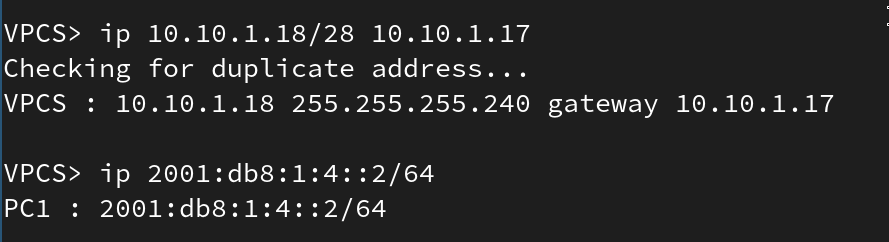
\includegraphics[width=\textwidth]{../images/image29.png}
    \captionof{figure}{Задание IP-адреса для PC1.}
    \label{29}
\end{center}

\begin{center}
    \centering
    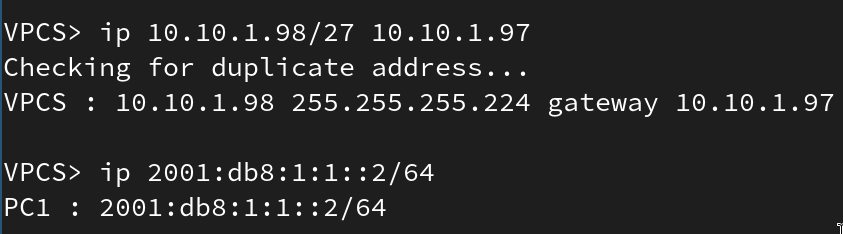
\includegraphics[width=\textwidth]{../images/image30.png}
    \captionof{figure}{Задание IP-адреса для PC2.}
    \label{30}
\end{center}

\item Настройка IP-адресов интерфейсов маршрутизатора \texttt{msk-dastarikov-gw-01} (рис. \ref{31}-\ref{34}):
  
\begin{center}
    \centering
    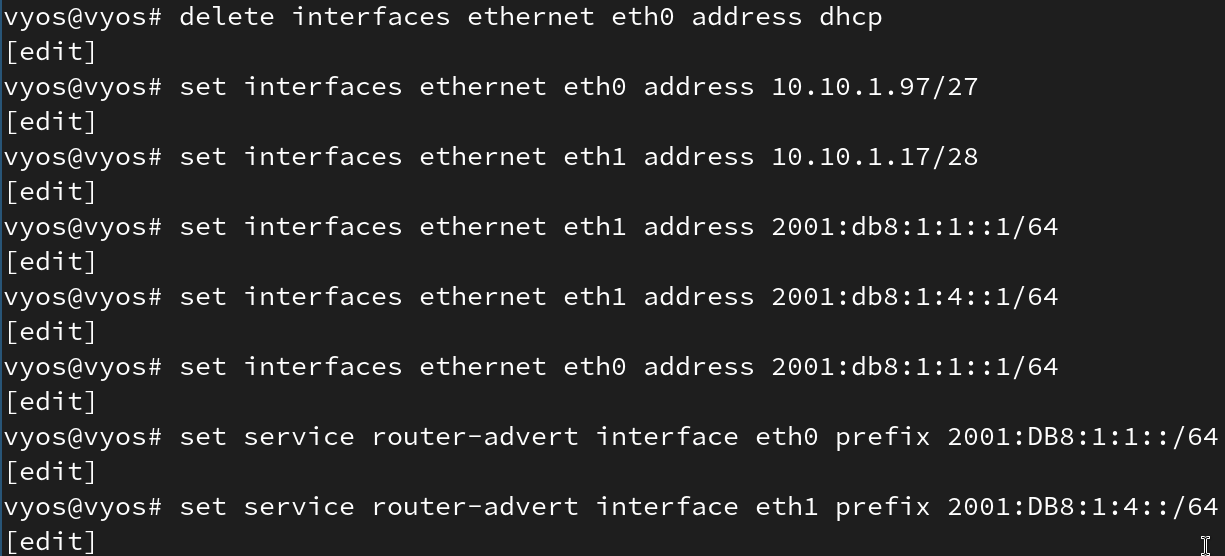
\includegraphics[width=\textwidth]{../images/image31.png}
    \captionof{figure}{Конфигурорование интерфейсов маршрутизатора.}
    \label{31}
\end{center}
  
\begin{center}
    \centering
    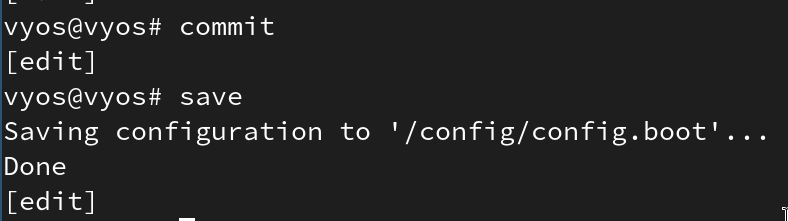
\includegraphics[width=\textwidth]{../images/image33.png}
    \captionof{figure}{Сохранение настроек.}
    \label{33}
\end{center}
  
\begin{center}
    \centering
    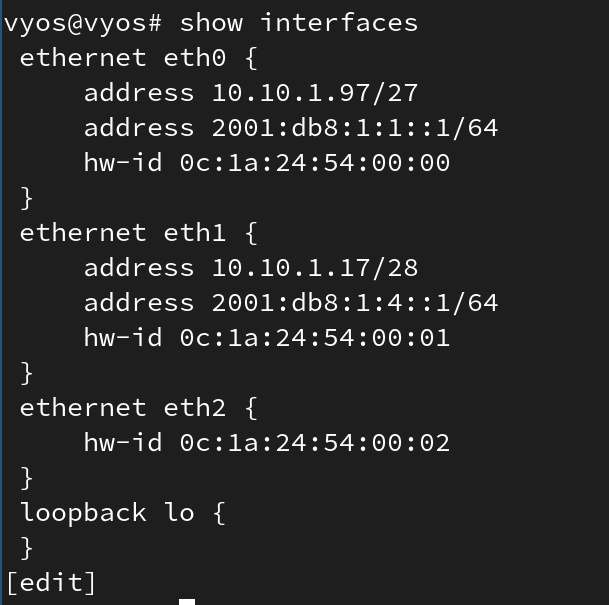
\includegraphics[width=\textwidth]{../images/image34.png}
    \captionof{figure}{Просмотр текущей конфигурации интерфейсов маршрутизатора.}
    \label{34}
\end{center}

\item Проверили подключение между PC1 и PC2 (рис. \ref{35} и \ref{36}):
    
\begin{center}
    \centering
    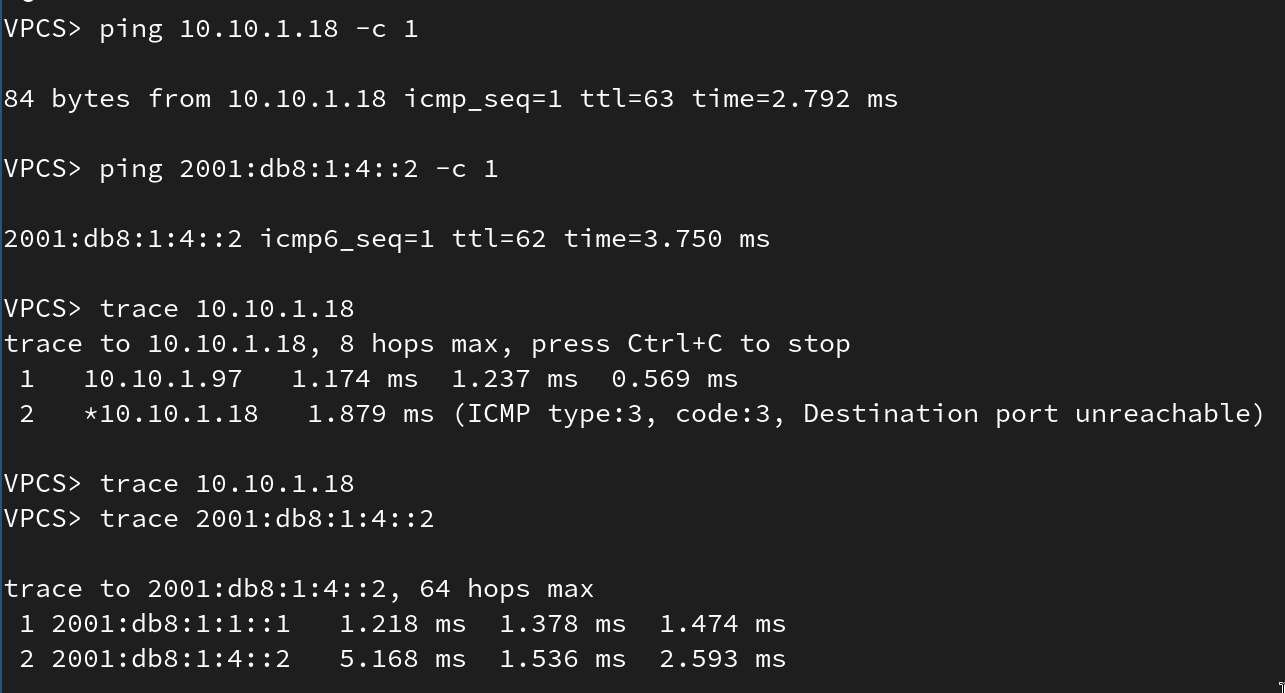
\includegraphics[width=\textwidth]{../images/image35.png}
    \captionof{figure}{Отправка эхо-запроса от PC1 к PC2.}
    \label{35}
\end{center}
    
\begin{center}
    \centering
    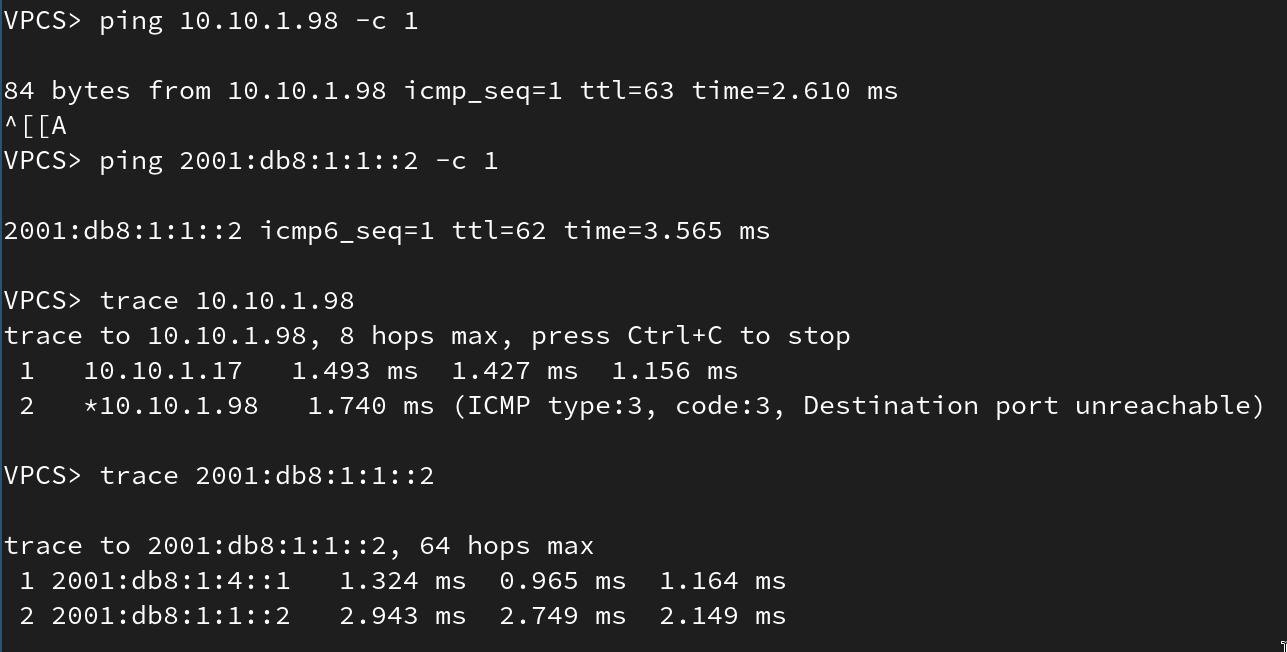
\includegraphics[width=\textwidth]{../images/image36.png}
    \captionof{figure}{Отправка эхо-запроса от PC2 к PC1.}
    \label{36}
\end{center}

\end{enumerate}

\section{Выводы}
В результате выполнения лабораторной работы изучили принципы распределения и настройки адресного пространства на устройствах сети.
\end{document}
